\title[JASA/draft]{Under-ice acoustic navigation using real-time model-aided range estimation}
\author{EeShan C. Bhatt}
\email{ebhatt@whoi.edu}
\affiliation{MIT-WHOI Joint Program in Oceanography/Applied Ocean Science \& Engineering, Cambridge and Woods Hole, MA, USA}
\affiliation{Department of Mechanical Engineering, Massachusetts Institute of Technology, Cambridge, MA}
\author{Oscar Viquez}
\affiliation{Department of Mechanical Engineering, Massachusetts Institute of Technology, Cambridge, MA}
\author{Henrik Schmidt}
\affiliation{Department of Mechanical Engineering, Massachusetts Institute of Technology, Cambridge, MA}

% \author{Author Four}
% \email{author.four@university.edu}
% \affiliation{Department2,  University2, City, State ZipCode, Country}

\preprint{Bhatt, JASA}   %  if you want want this message to appear in upper right corner of title page

\date{\today}

\begin{abstract}
The long baseline (LBL) underwater navigation paradigm relies on the conversion of recorded travel times into pseudoranges to trilaterate position.
For real-time operations, this conversion has assumed an isovelocity sound speed.
For re-navigation in post-processing, computationally and/or labor intensive acoustic modeling may be employed to reduce uncertainty driven by multipath arrivals.
This work demonstrates a real-time ray-based prediction method of the effective sound speed along a path from source to receiver to minimize vehicle position error.
\llabel{2.1} This method was implemented for a small scale AUV-LBL system in March 2020, in the Beaufort Sea, in total ice-covered conditions and a double ducted acoustic propagation environment.
The vehicle was successfully deployed and recovered.
\llabel{2.2} Given the lack of GPS data throughout the vehicle's mission, however, the pseudorange performance is first evaluated on connections between GPS-linked beacons.
The real-time ranging error between beacons is roughly 11 meters at distances up to 3 km.
But a consistent overestimation in the real-time method provides insights for improved eigenray filtering by the number of surface bounces.
An operationally equivalent pipeline is used to re-position the LBL beacons and re-navigate the AUV, using a modeled, historical, and a locally observed sound speed profile.
The median re-navigation error is 1.84 $\pm$ 2.19 RMS m.
The improved trilateration performance for suggests that this approach effectively extends the single meter accuracy of the deployed GNSS units into the water column. \llabel{2.3}
\end{abstract}

%% pacs numbers not used

\maketitle

% =========================================================================== %
% =========================================================================== %

\section{Introduction}
\label{sec:1}  
Autonomous underwater vehicles (AUVs) are increasingly capable platforms to explore and sample the ocean, particularly for remote and/or dangerous regions.
However, navigation uncertainty is a major challenge in considering AUVs as standard tools for oceanographic research.
While land and air-based robots utilize information from Global Navigation Satellite Systems (GNSS) to achieve stunning location accuracy and precision throughout the duration of their missions, AUVs cannot access GNSS fixes while underwater.
Therefore, underwater vehicles have relied on any combination of dead reckoning, hydrodynamic models, inertial navigation systems, doppler velocity logs, and acoustic baseline positioning systems for navigation \citep{paull_auv_2014}.
Limiting navigation error and drift requires an AUV to periodically stall on the surface and obtain a GNSS fix to reset its position error.
This foolproof method of self-positioning is undesirable for stealth, adverse weather conditions, and mission efficiency, and inaccessible in a GNSS-denied situation like an ice-covered environment.

% introduce LBL and precise statement of work
Of underwater acoustic navigation systems, long baseline (LBL) is the most GPS-like in style and scale, and most appropriate for mitigating drift without overburdening computation or payload size on the vehicle \citep{van_uffelen_global_2021}.
The state-of-the-art for LBL outsources depth to a pressure sensor and solves the two-dimensional localization problem with an isovelocity, linear scaling between one way travel time (OWTT) and range \citep{Eustice2006,Eustice2007,webster_advances_2012,Webster2009}.
This assumption is valid for short scale operations but oversimplifies propagation for larger and/or complex acoustic environments.
To achieve single meter, GNSS-like performance in a GNSS-denied environment, we demonstrate an embedded ray-based data processing algorithm to convert recorded OWTTs into pseudorange estimates.
This methodology was integrated onto the AUV \emph{Macrura}, deployed and recovered in the Beaufort Sea, in March 2020, during the Ice Exercise 2020 (ICEX20).
A physics-driven methodology that received an \textit{in situ} sound speed profile (SSP) was necessary despite the small operational domain because of the relatively high-risk mission environment\textemdash total under-ice conditions and a variable double ducted acoustic environment.

%% rest of the background, JASA style

% PNT
For consistency, we delineate specific definitions for timing, positioning, and navigation from \citet{Howe2019}.
\begin{enumerate}
	\item Timing is the ability to acquire and maintain accurate and precise time anywhere in the domain of interest within user-defined timeliness parameters
	\item Positioning is the ability to accurately and precisely determine one's location referenced to a standard geodetic system
	\item Navigation is the ability to determine current and desired position (relative or absolute) and apply corrections to course, orientation, and speed to attain a desired position anywhere in the domain of concern
\end{enumerate}
Thus, navigation is inherently in real-time and depends on positioning; positioning depends on timing.
We also suggest re-navigation and re-positioning as post-processed corollaries, which may include knowledge or processing capabilities not available \textit{in situ}.

% More about LBL navigation
While RAFOS floats championed one way ranging for re-positioning \citep{Rossby1986,duda_evaluation_2006}, the ability to do so for navigation was facilitated by \llabel{1.11} the advent of the WHOI Micro-Modem \citep{Singh2006} and synchronized clocks \citep{rypkema_one-way_2017}.
\llabel{1.3a}
AUV navigation efforts have achieved root mean square (RMS) localization error on the order of tens of meters relative to GNSS surface position over less than ten kilometers in shallow \citep{Eustice2007,Claus2018,kepper_mems_2017} and deep water \citep{Kunz2008,jakuba_long-baseline_2008,Webster2009}.
However, these efforts all used a nominal sound speed for travel time conversion and the vehicles were limited to shallower isovelocity regimes.

Localization algorithms that do consider environmental or acoustic uncertainty tend to focus on longer and larger experiments, where spatio-temporal variability cannot be ignored.
These methods have also been reserved for post-processing as they can be labor intensive, computationally heavy, and/or require additional information like contemporaneous data.
For example, gliders navigating with kinematic flight models and equipped with acoustic modems were later unambiguously associated with predicted ray arrivals, resulting in roughly a kilometer error and hundred meters uncertainty over basin scale propagation \cite{VanUffelen2013}.
A follow up study investigated how a single temporally and spatially averaged SSP could mitigate position error for a four month glider mission \cite{vanuffelen2016localization}.
\citet{Wu2019} cross correlate three days of real acoustic records with synthetic ones generated through ocean model snapshots from HYCOM \cite{chassignet_hycom_2007}.
While potentially applicable for various ocean states, this is reliant on model realism and impractical for real-time operations.
A ``cold start'' algorithm that does not require prior knowledge of track, position, or sound speed information inputs a four-dimensional ocean model, constrained by tomography data, into a range dependent ray code to isolate the last path detected in a full multipath pattern \citep{Mikhalevsky2020}.
Then, a representative group speed is solved for alongside position in a least squares fashion. 
This approach is able to re-position a floating hydrophone array with an error of 58 m and a standard deviation of 32 m based on six sources 129--450 km away but remains to seen for real-time navigation.

The ICEX20 AUV deployment necessitated an environmentally- and physically-driven relationship between recorded travel times and estimated pseudoranges due to the multipath uncertainty brought upon by an increasingly observed double ducted environment in the Beaufort Sea, which some refer to as the ``Beaufort Lens'' \citep{litvak2015,chen_spectral_2019,chen_temporal_2020}.

\llabel{2.1a}
Given that a lens introduces significant ray refraction, the Beaufort Lens is a shorthand for the spatio-temporal variability of the local temperature and sound speed maxima generally around 50 to 60 m in depth.
\llabel{2.4}
A neutrally buoyant layer of warm Pacific Summer Water creates a unique double ducted environment \textemdash the upper duct degrades signal coherence due to intensified ice interaction and the lower duct effectively traps sound for long range propagation \citep{Poulsen2016}. 
Modeling output \citep{duda_long-range_2019,duda_effects_2021} and experimental observations \citep{Ballard2020,Bhatt2021} suggest that, in the Beaufort Sea, the duct is persistent and widespread but not necessarily continuous; it and its acoustic effects can be non-existent, minimal, or drastic.
Transmissions in the upper duct, between the surface ice and the lens, experience minimal attenuation but degrade in signal coherence with repeated reflections under the ice.
In lower duct, between the lens and its conjugate depth in the Atlantic water, roughly 200 m, sound above 350 Hz is trapped near losslessly for long range propagation \citep{Poulsen2016}.

The Arctic, while remote, is the perfect place to demonstrate mature navigation technologies in real GNSS-denied conditions.
Thorough reviews of uncrewed vehicle operations in polar environments can be found in \citet{norgren2014unmanned} and \citet{Barker2020}; there is no comparable work in the Arctic for a short range AUV deployment in the Beaufort Lens.
Seminal \citep{brooke1981arcs,jackson1983autonomous,light1989autonomous,bellingham1995auv,hayes2002determining} and more recent AUV deployments \citep{,jakuba_long-baseline_2008,Kunz2008,Kukulya2010,Plueddemann2012,timmermans2013scales,fossum2021adaptive} witnessed the classical upward refracting sound speed profile that is amenable to an isovelocity assumption.

Of note, despite different platforms and scales, are recent glider deployments in the Canada Basin.
In 2014, in partially ice-covered conditions, a long range LBL system with WHOI Micro-Modems at 100 m exploited the lower duct for long range communication with two gliders \citep{Freitag2016,Webster2015}.
The sound speed value measured at the time of reception was used to estimate pseudorange in post-processing.
The beacon-to-beacon performance was excellent, achieving contact at ranges greater than 200 km with a position uncertainty of 40 m.
The beacon-to-glider performance, however, deteriorated due to missed contacts outside the duct, and was not described quantitatively.
In 2017, gliders were deployed in a region with no ice coverage \citep{Graupe2019}.
Ranges were linearly scaled by a statistical description of sound speed observations taken during the experiment, 1450 $\pm$ 6.5 m/s.
This resulted in an error of 550 m, which was reduced by a factor between 4 and 5, depending on the dive, using a post-processing acoustic arrival matching method.
Both cases exploit the lower duct for high fidelity communication at long ranges.
Unintuitively, the smaller nature of our deployment during ICEX20 is not a simplifying factor.
For source depths typical to vehicle operations, 30 to 200 m, a shadow zone spans from 2 to 6 kilometers in range \citep{schmidt_acoustic_2016}.

Compared to the previous small scale navigation efforts, the approach in this paper integrates real-time model-aided data processing to estimate a representative sound speed along a path from source to receiver, leveraging climatology, \textit{in situ} data, and fast acoustic modeling.
The paper is organized as follows.
Section \ref{sec:icex20} details the experimental approach and conditions during ICEX20.
Given that there is no GNSS ground truth for the vehicle position while underway, we first evaluate the real-time ranging performance of GPS-linked beacon-to-beacon communication events in section \ref{sec:realtime}.
Section \ref{sec:post} uses insights from field data to introduce a new ray filtering algorithm to improve range estimation.
Section \ref{sec:trilat} emulates the real-time processing pipeline to re-position beacon-to-beacon events and re-navigate AUV \emph{Macrura}.

\clearpage
\section{Overview of the ICEX20 experiment}\label{sec:icex20}

The results from this paper derive from data taken while deploying the AUV \emph{Macrura}, a custom Bluefin-21, during the Ice Exercise 2020 (ICEX20), in the Beaufort Sea, from March 8th to 11th.
The AUV deployment was supported by the Integrated Communication and Navigation Network (ICNN) \citep{schneider_self-adapting_2020,Randeni2020,randeni_high-resolution_2021} a specialized implementation of the LBL solution.
The ICNN was initially developed via numerous virtual experiments to ensure robust algorithms and interfaces between different hardware components. 
The simulation capabilities are largely physics-driven with a modular system of systems approach\textemdash an environmental simulator with sub-components for the ocean, including Arctic ice drift and ocean acoustic propagation; a vehicle simulator with sub-components for vehicle dynamics and navigation; a topside hardware simulator and acoustic communications simulator, both with a software-only configuration and a hardware-in-the-loop version \citep{schneider_netsim_2018}.
The virtual environment similarly emulates the interfaces between the real components to test the entire software pipeline.

\subsection{The Integrated Communication and Navigation Network}

\begin{figure}[h!]
	\centering
	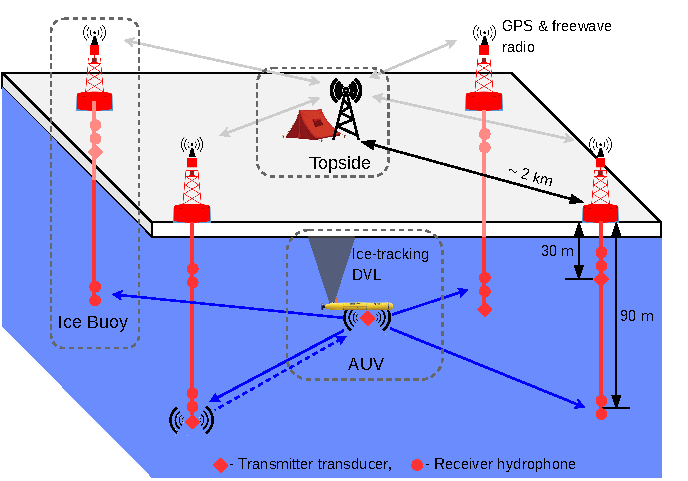
\includegraphics[width=0.8\columnwidth]{figs/Fig2.pdf}
	\caption{A schematic overview of the Integrated Communication and Navigation Network (ICNN), which provides joint data-transfer and tracking between AUV and a human decision maker at Topside.}
	\label{fig:icnnOverview}
\end{figure}

The ICNN is comprised of four ice buoys in a loose rectangle, roughly 2 km away from a central ice camp with a topside computer, as shown in Fig.~\ref{fig:icnnOverview}.
Each ice buoy is outfitted with a Garmin GPS 18x, with a pulse-per-second rising edge aligned to 1 microsecond and a spec sheet accuracy of 3 m, 95\% of the time.
The AUV and each ice buoy are outfitted with a WHOI Micro-Modem \citep{Singh2006}, with a four-element receiver array, a single transmitter, and one-tenth of a millisecond resolution.
\llabel{1.6a} Acoustic messages were sent with a 10 kHz carrier frequency, 5 kHz bandwidth, and phase-shift keying (PSK) modulation on a time-division multiple access schedule with a thirty-second cycle, giving room for two-way communication throughout the mission volume.
The receive and transmit elements were split between shallow and deeper depths\textemdash 30 and 90 m\textemdash to provide better coverage across the shadow zone.
While each buoy only has one transmit depth, all buoys have both receive depths but the active receive layer is consistent across all buoys. \llabel{1.12}
The design of the ICNN enables a self-adapting network to transmit and receive at the optimal depth to maintain contact with the AUV \citep{schneider_self-adapting_2020}.
The buoys do not encompass the full horizontal range of the vehicle but are positioned to minimize overlap in trilateration for spherical positioning \citep{deffenbaugh1996posit}.

To balance competing uses of the acoustic channel, the network uses a single synchronized digital communication packet to provide both tracking and data to the operator.
\begin{enumerate}
\item The AUV, running an ice-tracking DVL and an onboard hydrodynamic model, broadcasts its perceived location on a scheduled, time-synchronized message via WHOI Micro-Modem
\item Four ice buoys, each outfitted with a WHOI Micro-Modem, receive messages from the AUV and send that information over freewave radio to a Topside computer
\item The topside computer converts travel times into pseudorange estimates using a stochastic embedded prediction of the horizontal group velocity via BELLHOP ray tracing code \citep{Porter2011} using a sound speed profile provided by an updatable Virtual Ocean \citep{schneider_netsim_2018,bhatt_embedded_2022}
\item The topside computer calculates a new position by trilaterating the range estimates
\item The position differential, not the absolute position, is broadcast to the vehicle to update its navigation solution and be robust to latency and intermittency
\end{enumerate}

In the face of GNSS-denied navigation, this approach was anecdotally successful, as shown in Fig. \ref{fig:vehicleRecovery}.
The AUV \emph{Macrura} was deployed through a hydrohole from an ice camp but recovered through an emergency hydrohole.
A random disk error stalled \emph{Macrura} underneath the ice but did not prevent it from transmitting its location.
Due to an incoming storm, a team placed a physical marker on the ice at the location.
Three days later, \emph{Macrura} was found within a meter of the marker.
We view the emergency recovery as qualitative proof of the robustness of this navigation approach.
Nonetheless, this paper specifically addresses the third and fourth steps\textemdash the conversion of travel times into pseudoranges and its effect on trilateration.
By focusing on pseudorange estimates between GPS-tracked beacons, and re-running the trilateration pipeline, the results are decoupled from all other mechanisms in the ICNN.

\begin{figure}[h!]
	\centering
	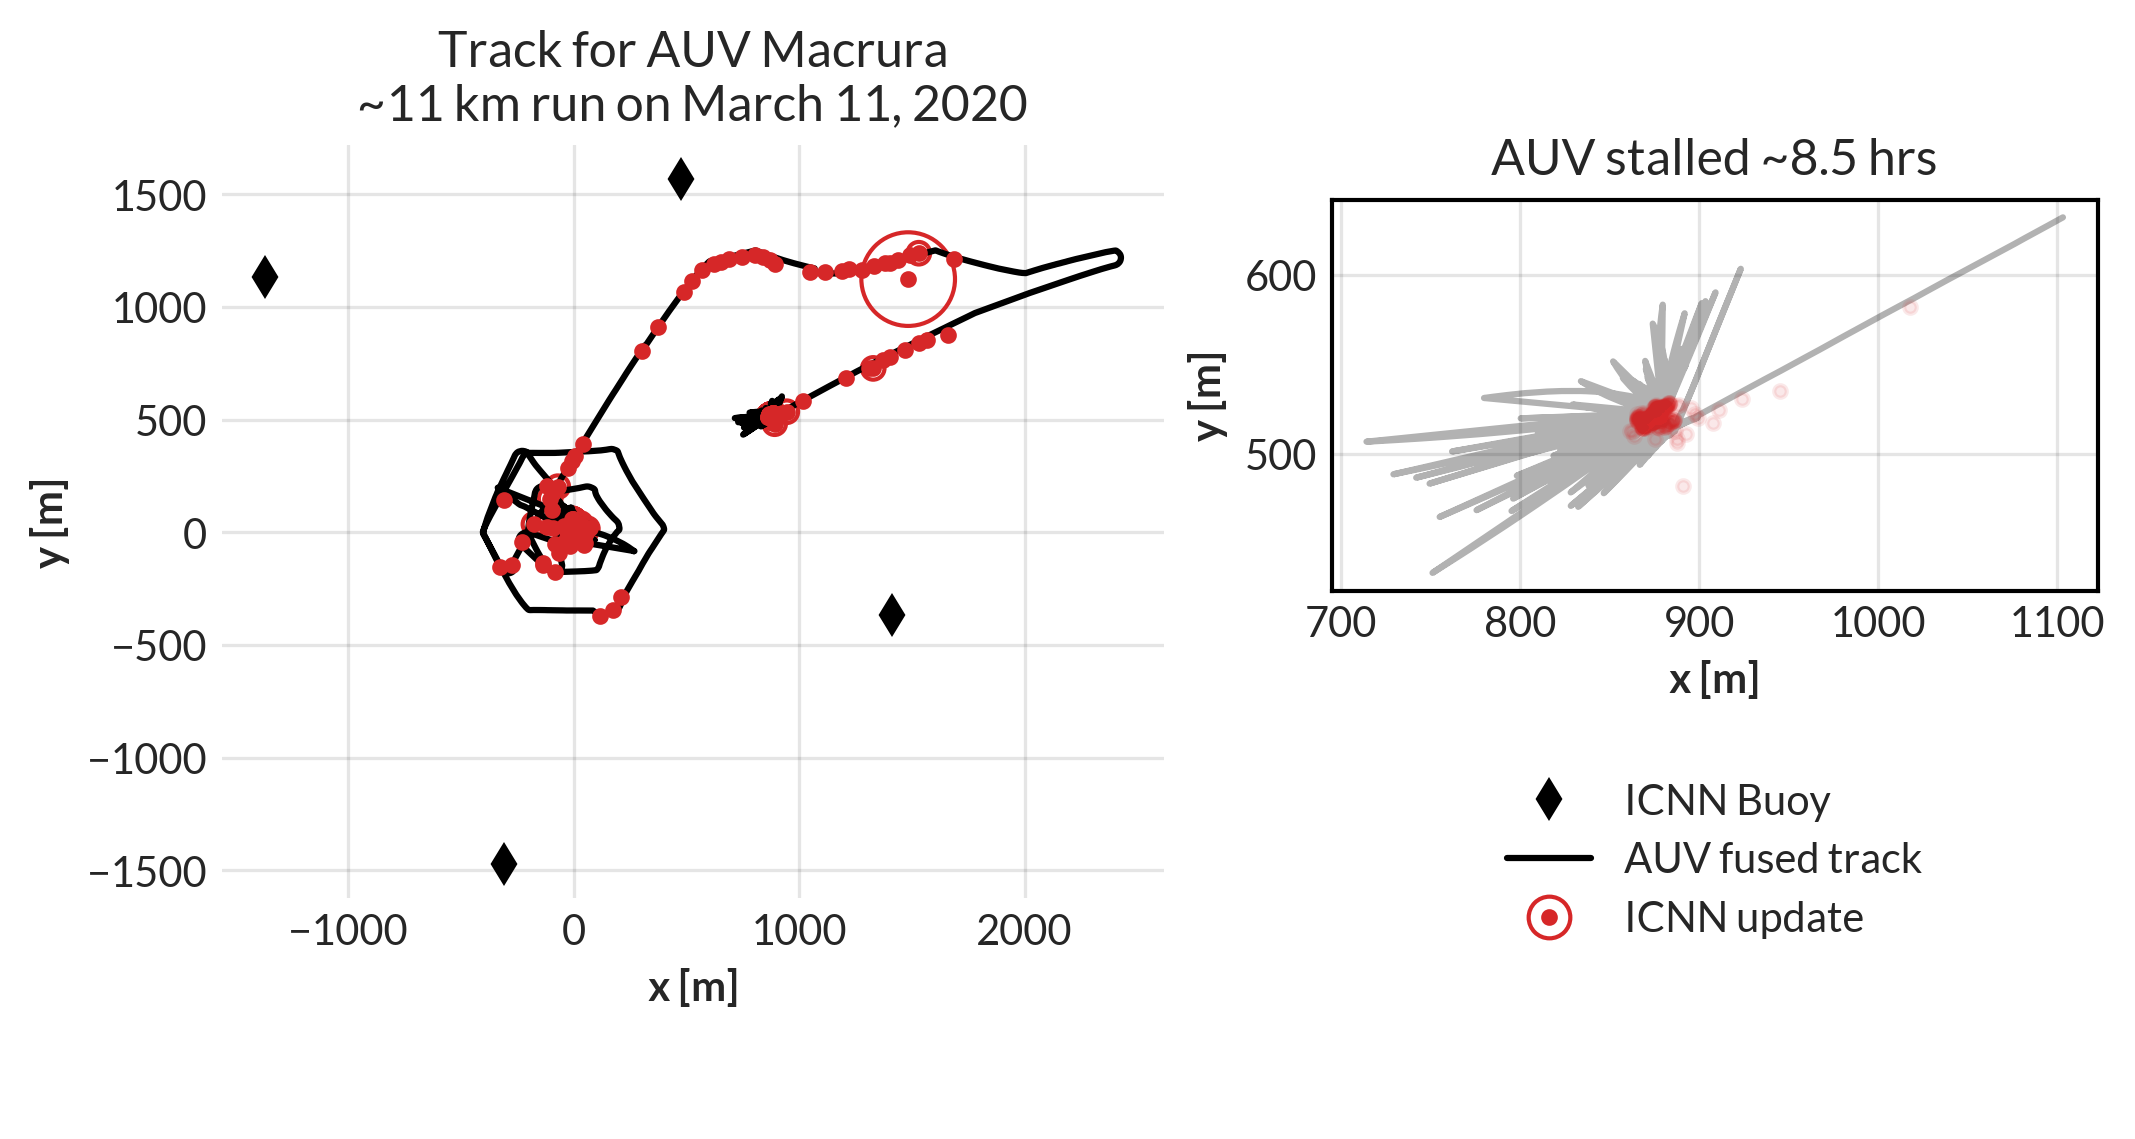
\includegraphics[width=0.7\columnwidth]{figs/auv-track-update.png} \hfill
	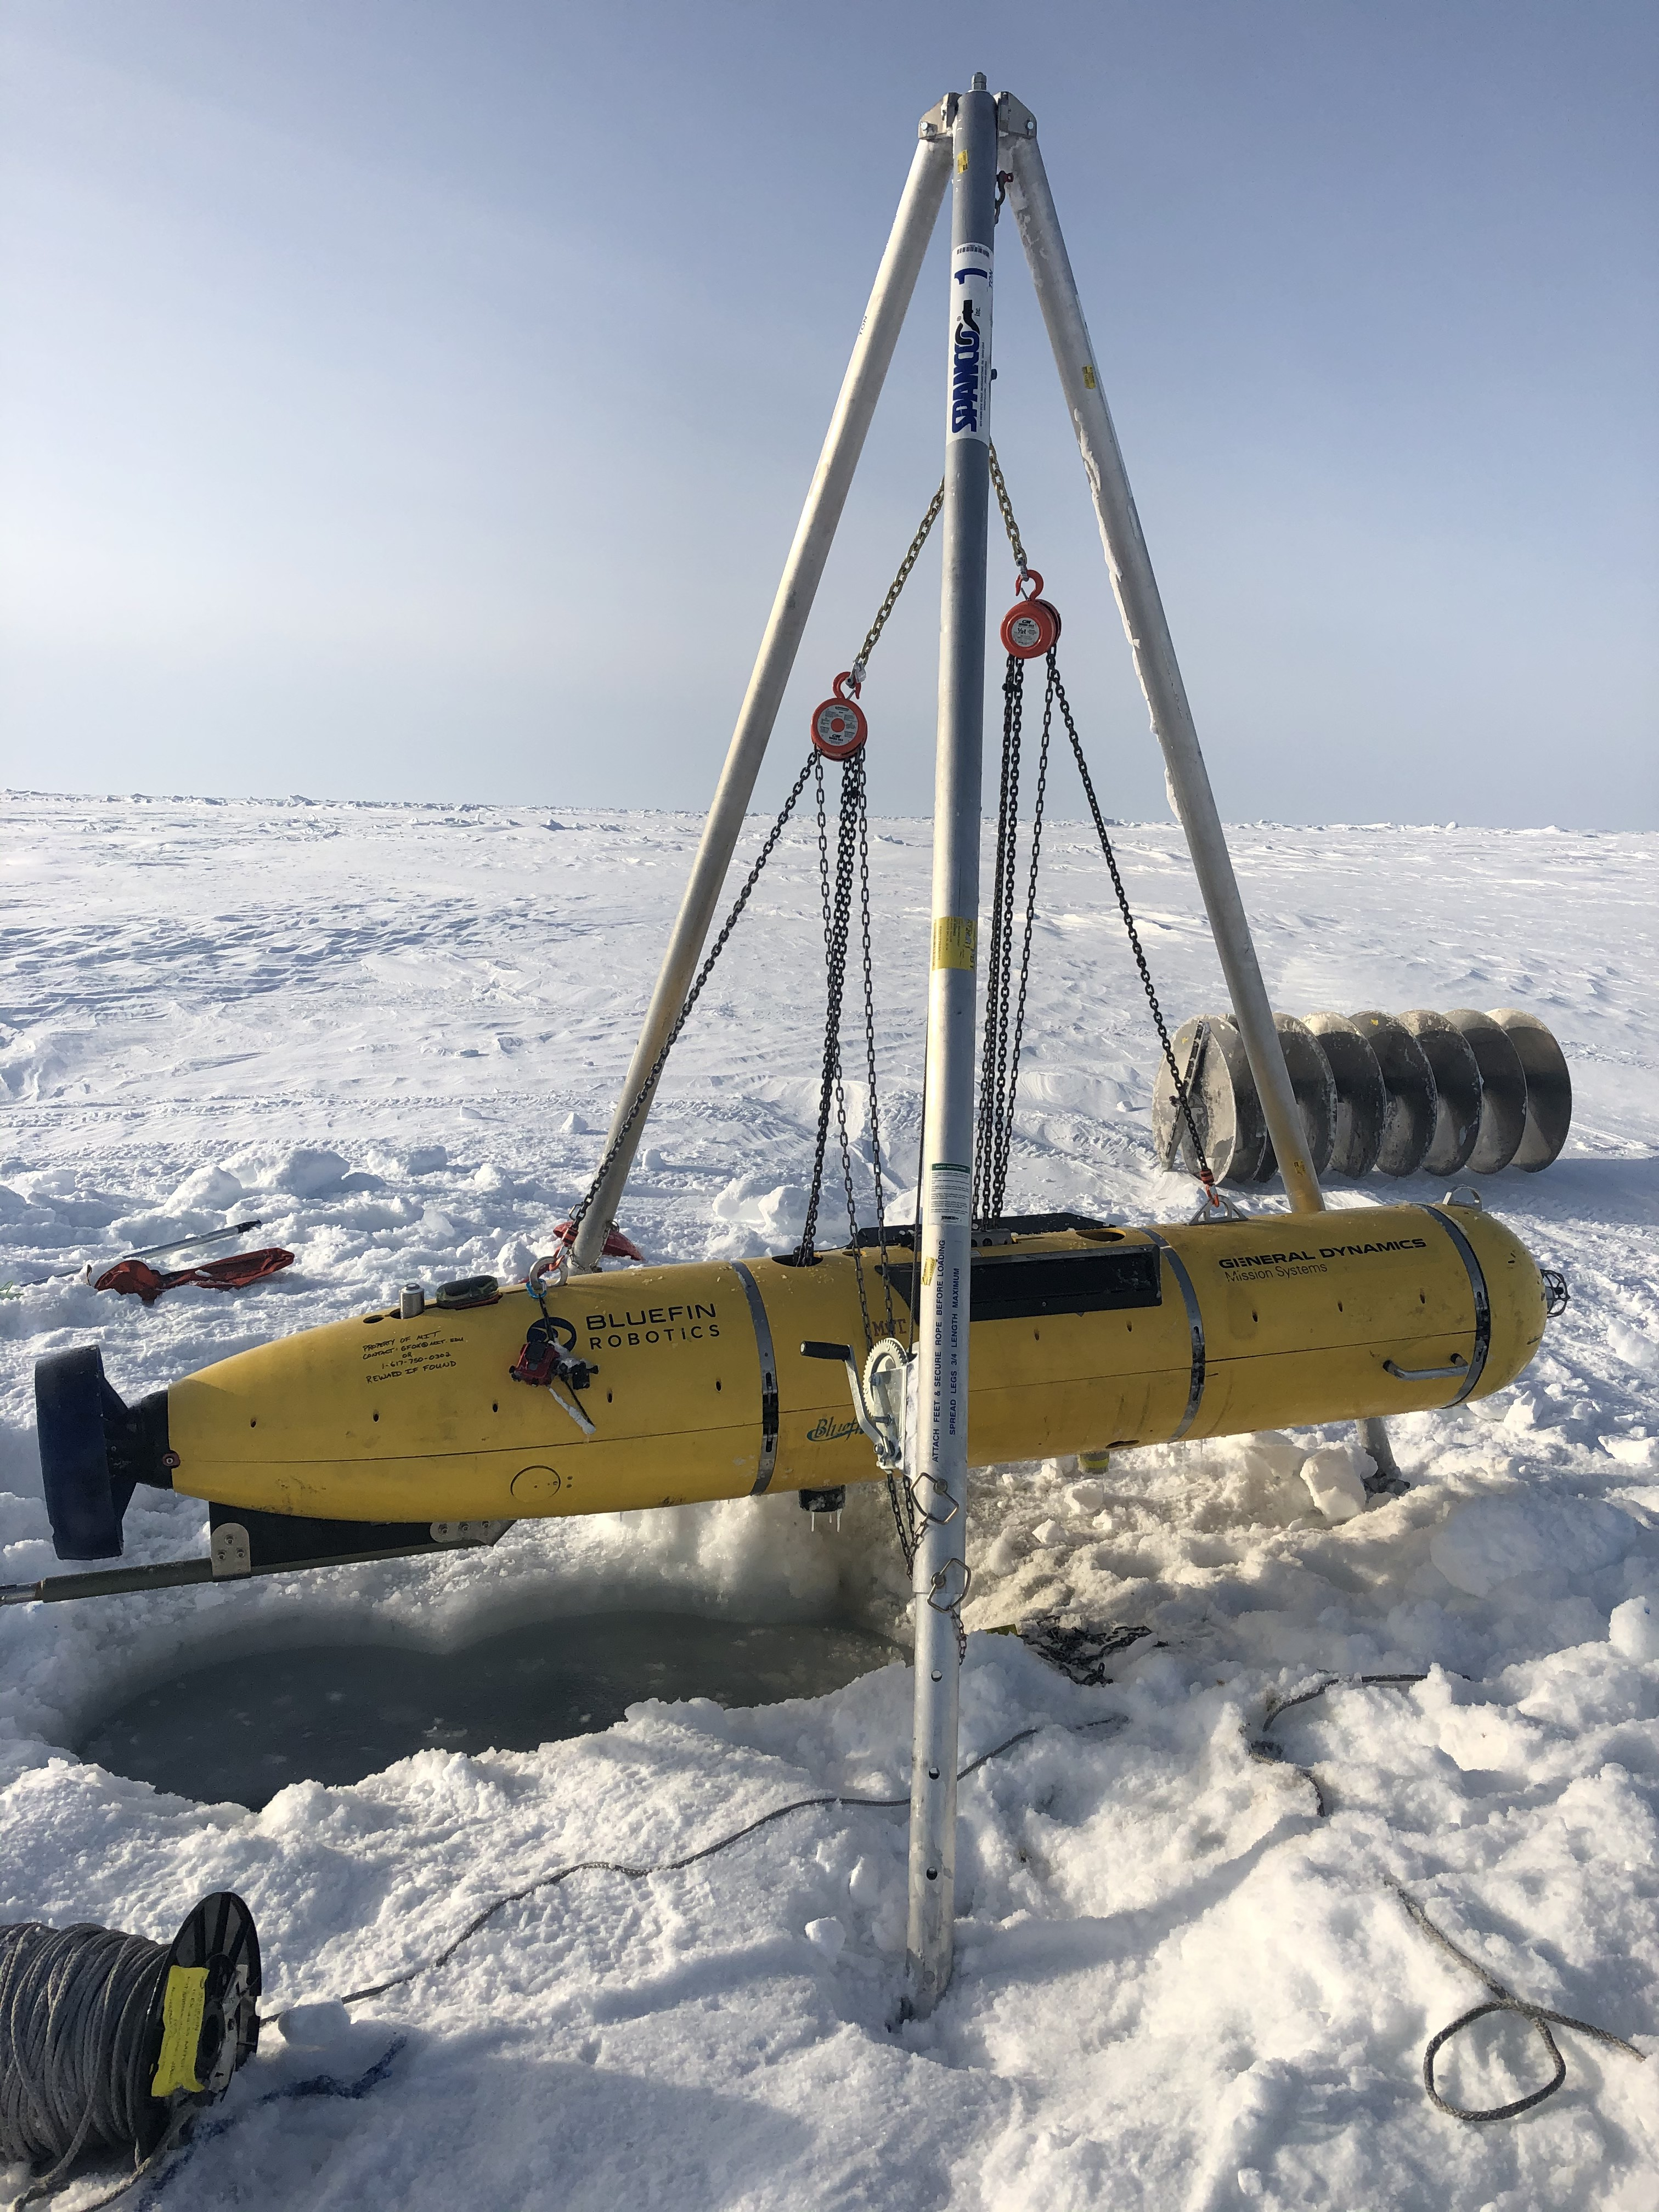
\includegraphics[width=0.28\columnwidth]{figs/Fig1.jpg}
	\caption{The under-ice mission track for AUV \emph{Macrura}, including the position updates as it stalled underneath the ice overnight. A marker was placed on the ice at the vehicle's estimated self-location. It was recovered after a three day storm within a meter of the marker.}
	\label{fig:vehicleRecovery}
\end{figure}

\subsection{ICEX20 sound speed conditions}

An important component to our navigation solution is an accurate estimation of a representative SSP for the ocean volume.
Previous field experience, during the Ice Exercise 2016 (ICEX16), demonstrated the negative effects of the Beaufort Lens on tracking and communication \citep{schmidt_acoustic_2016}.
Fig. \ref{fig:sspExpectation} shows historical, modeled, and \textit{in situ} sound speed data for both ICEX16 and ICEX20.
These three input streams were selected to mirror the information available on a submarine (personal conversation with LT B. Howard and LT CDR D. Goodwin). \llabel{1.8}
In the field, the SSP information was shared with the vehicle via basis representation compression on a lightweight digital acoustic message \citep{bhatt_embedded_2022}. \llabel{2.7}
All modeled data comes from HYCOM \cite{chassignet_hycom_2007}, which does not seem to capture the forcing mechanisms that cause the Beaufort Lens.
For ICEX16, the data-driven profile was sourced from nearby Ice Tethered Profilers (ITP) after the field experiment \cite{Krishfield2008,toole_ice-tethered_2011} and exhibits a fairly low lens; the historical profile is from the World Ocean Atlas.
For ICEX20, the chosen weights (data-driven) profile derives from an estimate of initial CTD casts taken on site, showing an intense warm water intrusion; the baseline (historical) profile, showing moderate ducted conditions, comes from the average of March 2013 ITP data.
This month best matched sea ice and sound speed conditions at the beginning of ICEX20 \citep{bhatt_embedded_2022}.
It is important to note that all profiles that do show the Beaufort Lens do so with different local sound speed maxima at different depths, reflective of the wide range of lens properties observed for all ITP data in the region. \llabel{2.5}
The variability of the lens height and prominence is the main reason an updatable SSP was integrated into the ICNN solution.

\begin{figure}[h!]
	\centering
	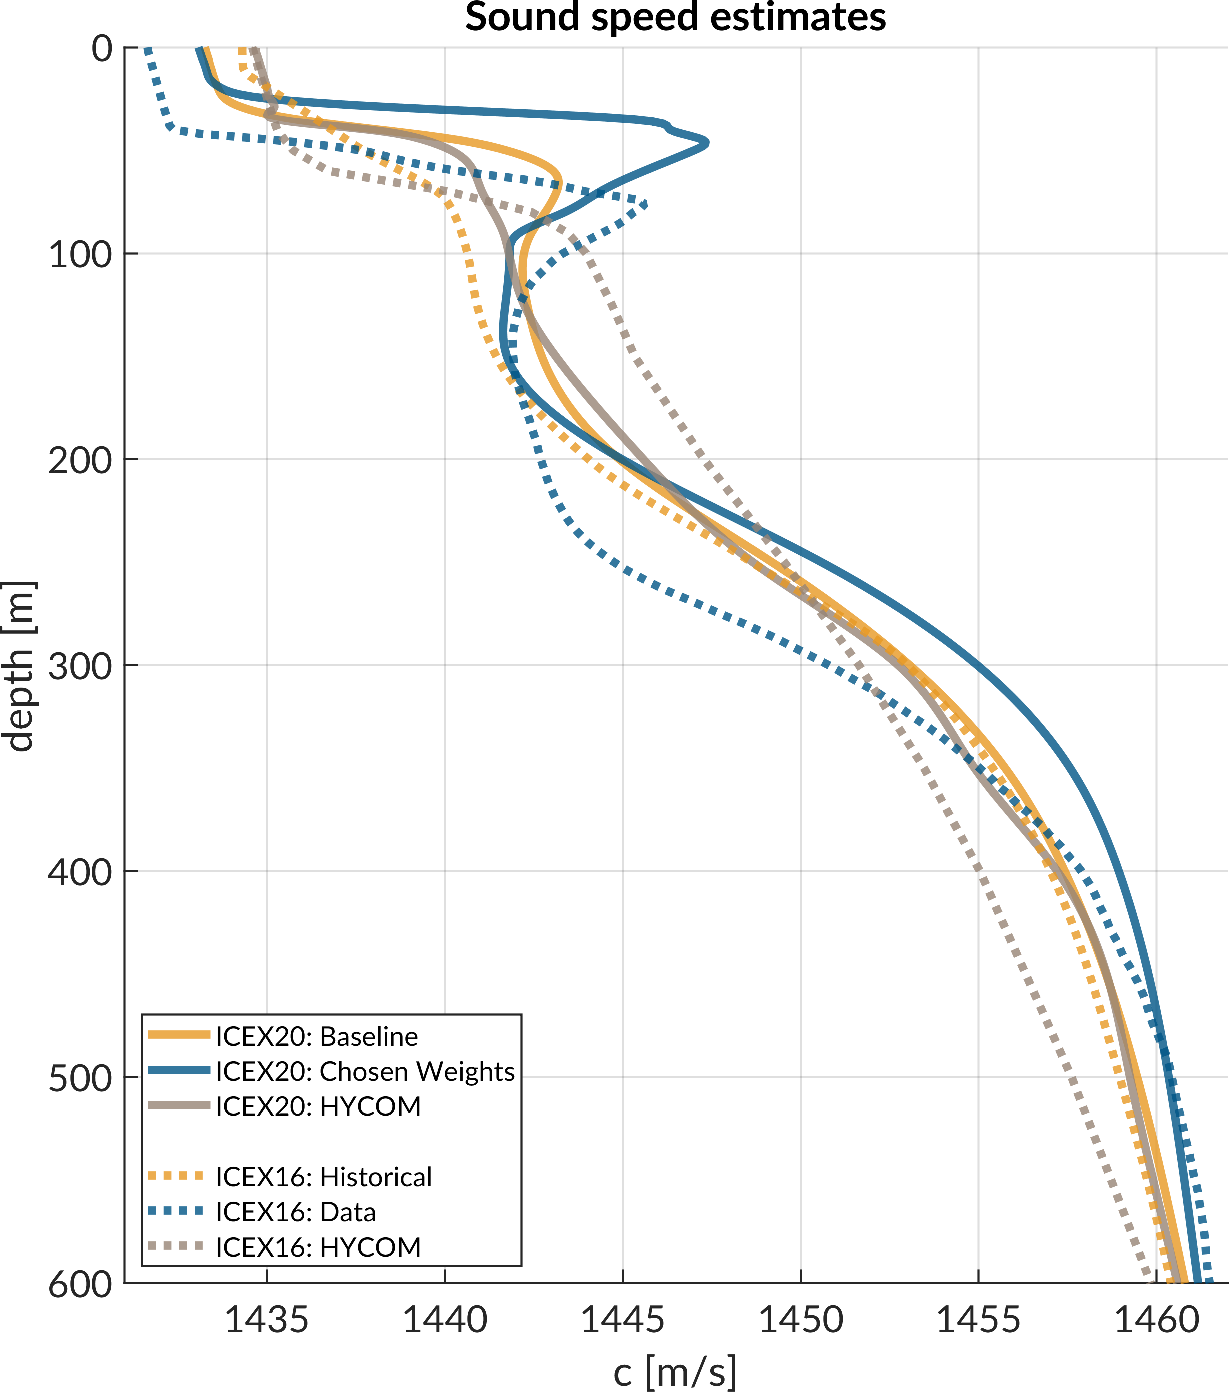
\includegraphics[width=\reprintcolumnwidth]{figs/ssp-gvel-icex20-icex16.pdf}
	\caption{Sound speed conditions for historical (baseline), data (chosen weights), and HYCOM model for both ICEX16 and ICEX20.}
	\label{fig:sspExpectation}
\end{figure}

During ICEX20, the HYCOM profile was available but never deployed. \llabel{1.14}
For post-processing comparison, we introduce both the HYCOM profile and an isovelocity case, 1441.8 $\pm$ 3.7 m/s, as the mean and standard deviation of the observed sound speed profile over the first 200 m.
This is a contrived value taken in the style of \citet{Graupe2019} for the sake of comparison; the default value in the LAMSS simulator, which was not environmentally informed nor used during ICEX20, was 1430 m/s.

\clearpage
\section{\label{sec:realtime} Real-time pseudorange analysis}

Because the vehicle's navigation solution during a mission can only be evaluated on the basis of the error estimates sent, a sister experiment for validating the real-time ranging approach was implemented.
Ice buoy modems were run as ``virtual vehicles'' at a fixed depth, receiving position updates from the other beacons as well as a camp site modem lowered to 20 m. \llabel{1.13}
Fig. \ref{fig:overview} shows successful events sorted by source depth.
\llabel{1.10}
In this analysis, we assume there is insignificant displacement between the GNSS puck surface expression and subsurface modem; this is supported by unusually low observed ice drift rates, just 0.7 cm/s on average throughout the mission.

\begin{figure}[h!]
  \centering
  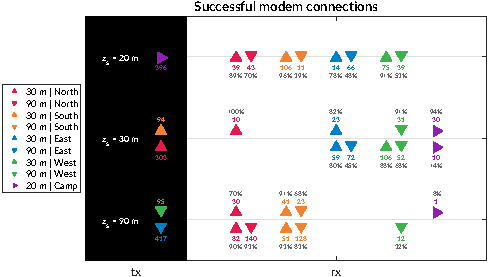
\includegraphics[width=\columnwidth]{figs/modem-chart.pdf}
  \caption{An overview of the modem experiment by source and receiver depth and position. The black column on the left, $tx$, shows the source depth, $z_s$, with the total number of transmissions. The column on the right, $rx$, shows the receivers with the number of successful decodings and the percent success rate, defined as the ratio of decoded to detected. The orientation of the triangles\textemdash sideways, upwards, and downwards\textemdash corresponds to depths of 20, 30, and 90 m.}
  \label{fig:overview}
  \end{figure}

\subsection{Minimal bounce criteria (MBC)}

\llabel{1.5} The fundamental challenge to implement GNSS-like navigation, especially in an acoustically complex propagation environment, is characterizing a single sound speed to compensate for the effects of ray refraction and reflection.
The use of the acoustic modem network for tracking relies on the accurate estimates of travel times between the submerged platform and LBL beacons, supported by clock synchronization and a pre-determined scheduling of acoustic events.
\llabel{2.9} For the Beaufort Lens in particular, the strong multipath effects make it virtually impossible to deterministically predict the modem's detected arrival time.

Instead, for each individual modem $i$, an embedded stochastic tracking framework is used to provide a running estimate of the effective sound speed $c_{i,j}$ for the conversion from travel time to range from modem $j$, with the ultimate goal of matching the implied horizontal effective sound speed, i.e., the GPS-recorded distance between two nodes divided by the modem-recorded one way travel time between them. 

\llabel{2.10} In the ICEX20 configuration, the acoustic tracking is running on the topside computer, which controls the ICNN.
Here we assume that the effective sound speeds $c_{i,j}$ are smoothly varying over the course of a vehicle mission, i.e., with respect to range, mission time, and the thirty-second frequency.

\llabel{1.15} When the topside tracking framework receives a message, with a time delay, $\Delta t$, it will request a new estimate for $c_{i,j}$ along with its standard deviation.
The effective sound speed is predicted using the vehicle's reported depth and the extrapolated navigation solution for range, $\hat{r}$, as inputs to the ray tracing program, which returns an impulse response estimate in the form of ray travel times $dt_{j}$ and amplitudes $a_{j}$.

\llabel{2.11} The initial call to BELLHOP is over a local grid centered at the range and depth posited by the onboard tracking solution.
The grid, compared to a point solver, adds redundancy in resolving the actual multipath structure for a reliable acoustic path without overtaxing onboard computational time and memory.
It is initialized as 11 $\times$ 11 points spanning 10 m horizontally and 20 m vertically.
The horizontal dimension reflects the accumulated vehicle position error given a thirty-second communication cycle; the vertical dimension reflects how, computationally, eigenrays of the same timefront seem to stack vertically in the water column. \llabel{1.17}
For each grid point, BELLHOP produces a number of arrivals resulting from multiple propagation paths.
Using only the $N_0$ rays with neither surface nor bottom bounces, it will then estimate the current effective sound speed $c$ from a power weighted average of the ray travel times,
\begin{equation}
c = \frac{\hat{r} \sum_{n=1}^{N_{0}} a_{n}^{2}}{\sum_{n=1}^{N_{0}} dt_{n}a_{n}^{2}} ~, 
\end{equation}
and the associated weighted standard deviation,
\begin{equation}
\sigma_{c} \simeq \sqrt{\frac {\sum_{n=1}^{N_{0}} (dt_{n}-\hat{r}/u)^{2}a_{n}^{2}}{ \sum_{n=1}^{N_{0}} a_{n}^{2}} } \frac{u^{2}}{\hat{r}}
\end{equation}
If no direct paths exist, i.e. $N_{0}=0$, then the effective speed is computed using the same algorithm for the ray arrivals with one bounce, and so on.

Finally, the pseudorange is calculated simply as
\begin{equation}
r_{i,j} = c_{i,j} \Delta t_{i,j} 
\end{equation}

Thus the MBC method assumes the signal detected by the modem will be dominated by a set of paths with the least number of boundary interactions.
Importantly, this stochastic, ensemble method for group velocity calculation can run in real-time, appearing to be orders of magnitude faster than other post-processing methods which seek to determine the specific ray itself that best matches a prominent indicator from the arrival structure.
The BELLHOP simulation that runs this calculation uses 3600 rays with launch angle fan of -60 to 60 degrees, a representative depth dependent sound speed profile, and a range dependent bathymetry. \llabel{1.13}

\subsection{Pseudorange error metrics}

The sister modem experiment generated 811 beacon to beacon communication events with their own real-time MBC group velocity predictions.
Given the complexity of the ICNN system, this experiment did not collect an exhaustive set of data across all buoy, source depth, receive depth, and sound speed combinations.
\llabel{1.18} The algorithm generally overestimates pseudoranges because it resolves the effective sound speed for the most direct path.

\begin{figure}[h!]
  \centering
  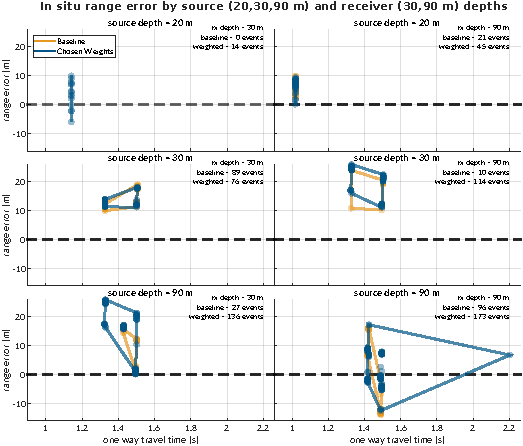
\includegraphics[width=\columnwidth]{figs/range-error-insitu.pdf}
  \caption{The real-time range error by source (rows: 20, 30, and 90 m) and receiver (columns: 30 and 90 m) pairings for both sound speed estimates used during ICEX20. The amount of communication events is notated in the top right of each panel. The dashed line indicates no range error, and the boundary drawn indicates scope of the range error as a function of one way travel time.}
  \label{fig:range-error-insitu}
\end{figure}

Fig. \ref{fig:range-error-insitu} shows the range error boundary for both SSP inputs used in ICEX20.
A promising sign that the MBC method adapts sound speed somewhat intelligently is the lack of error growth as travel time increases.
\llabel{1.28}
The baseline SSP (n=243 events) has an absolute pseudorange error of 11.38 $\pm$ 4.23 m; the weighted SSP (n=568), 11.36 $\pm$ 8.12 m.
The discrepancy between these two is largely due to outlier events only contained in the weighted SSP set.
Where there is overlap between sound speed conditions used for the real-time MBC, the pseudorange error difference is no more than a few meters.
The overarching results show that sound speed estimates derived from eigenrays for a local grid, as opposed to a singular point, are accurate enough to support vehicle navigation.
While the NBC looks for just the least complex multipath, the high density of launch angles almost always guarantees a direct path.
Nonetheless, the consistent overestimation of pseudorange invites further analysis into acoustic arrival matching.

\subsection{Eigenray identification for beacon-to-beacon events} \label{sec:eigenrays} \llabel{1.6b}

Accounting for ice movement between beacons creates nominal ranges with small variability.
Figs. \ref{fig:raytrace-zs20}, \ref{fig:raytrace-zs30}, and \ref{fig:raytrace-zs90} show eigenrays for three sound speed environments for source depths of 20, 30, and 90 m, respectively.
Eigenrays were initially found using the built-in BELLHOP protocol with a launch angle fan of 2400 rays between -60 and 60 degrees.
Separately, recorded travel times between beacons were clustered with 1 millisecond boundaries such that some source-receiver pairs had multiple, distinct travel times to approximate.
The BELLHOP eigenray returns\llabel{2.8} were then filtered such that one was selected per travel time cluster, in the hopes that the eigenray will converge to the receiver locations for the most realistic sound speed input. \llabel{1.16}
It should be noted that bottom bounces were recovered but filtered out.
The three source depths create distinct ray geometries with respect to the three sound speed inputs.

\subsubsection{Source depth of 20 m}
\begin{figure}[ht!]
  \centering
  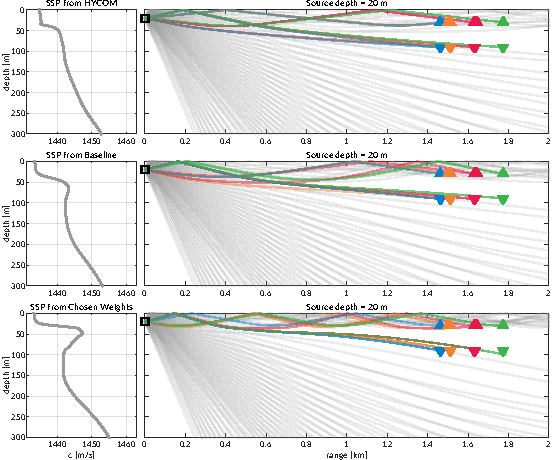
\includegraphics[width=\columnwidth]{figs/raytrace-3env-zs-20.pdf}
  \caption{Eigenrays for beacon-to-beacon events for each sound speed with a nominal source depth of 20 m over a total ray fan in gray. The beacons are highlighted in color/marker coding in Fig. \ref{fig:overview}.}
  \label{fig:raytrace-zs20}
\end{figure}

For a source at 20 m in depth, shown in Fig. \ref{fig:raytrace-zs20}, reliable eigenrays are found for all sound speed inputs.
Rays refract upwards and neatly intersect with the shallow and deep receiver locations between 1.5 and 1.8 km in range.
However, the ray paths for the shallow receivers change both in the number of surface interactions and where the surface interactions occur with respect to range across the SSPs.
As the Beaufort Lens strengthens, the chosen paths to the second farthest shallow buoy (North, in red) interact with the surface more and become distinct.
The weighted SSP shows the most interesting effects for the deeper receivers.
The ray paths all interact with the surface and the eigenrays for the Northern (red) and Western (green) buoys are in fact the same ray.

\subsubsection{Source depth of 30 m}
\begin{figure}[ht!]
  \centering
  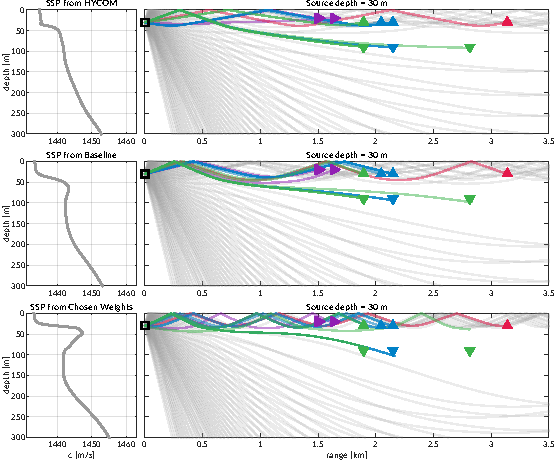
\includegraphics[width=\columnwidth]{figs/raytrace-3env-zs-30.pdf}
  \caption{Eigenrays for beacon-to-beacon events for each sound speed with a nominal source depth of 30 m over a total ray fan in gray. The beacons are highlighted in color/marker coding in Fig. \ref{fig:overview}.}
  \label{fig:raytrace-zs30}
\end{figure}

The ray geometries from the 30 m source, shown in Fig. \ref{fig:raytrace-zs20}, show a similar degradation of eigenray identification with increased ducting.
Receptions span 1.5 to 3.2 km.
Once again, eigenrays for HYCOM and the baseline SSP are visually appropriate.
Rays for the weighted SSP show how the surface channel intensifies ice interactions and how the shadow zone denies reliable acoustic paths.
Pointedly, the increasing number of surface reflections to the farthest shallow buoy (North, in red) crystallize the MBC's tendency for overestimation.
For the HYCOM, baseline, and weighted SSP inputs, the most appropriate eigenrays show 2, 3, and 4 surface interactions.

\subsubsection{Source depth of 90 m}
\begin{figure}[ht!]
  \centering
  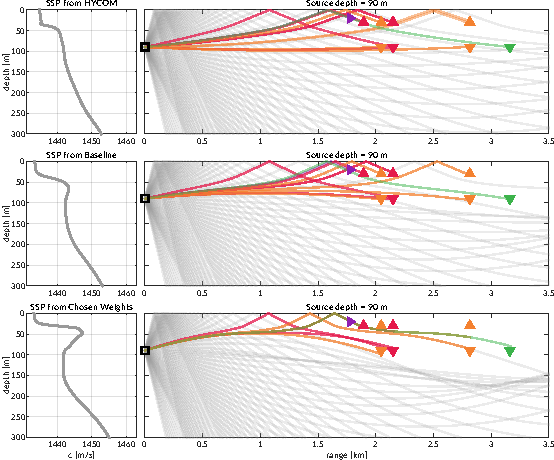
\includegraphics[width=\columnwidth]{figs/raytrace-3env-zs-90.pdf}
  \caption{Eigenrays for beacon-to-beacon events for each sound speed with a nominal source depth of 90 m over a total ray fan in gray. The beacons are highlighted in color/marker coding in Fig. \ref{fig:overview}.}
  \label{fig:raytrace-zs90}
\end{figure}

Lastly, Fig. \ref{fig:raytrace-zs90} shows ray geometries from the 90 m source, elucidating a different extent of the shadow zone. 
While the receiver locations are similar to that of the 30 m source depth, the deeper source depth effectively negates the upper duct and places the upper (and some of the lower) receivers in unreliable acoustic paths.
The HYCOM eigenrays still show the most reliable acoustic paths that deteriorate with increasing ducted conditions.
The lack of direct paths from the observed SSP further points out the shortcomings of the MBC approach.

The goal of the MBC algorithm was to provide a reliable, physically intuitive interpretation of the acoustic propagation without taking on the additional burden of regularly identifying specific paths that may connect any given source-receiver pair in the network.
While it was unlikely to resolve multipath arrivals that triggered successful modem detection, an isovelocity approach would have provided no adaptivity against source and receiver depth differences.
\llabel{2.14}
Its performance was adequate for vehicle navigation and would have likely sufficed if it were not for the prominence of the duct observed relative that of other model and data products.

\clearpage
\section{\label{sec:post} Post-processed pseudorange analysis}

From all events recorded during the modem test experiment, there are 1242 successfully decoded beacon-to-beacon events.
Thus, a post-processing analysis that emulates the real-time navigation engine was run to overcome the unequal distribution of communication events with respect to depth, range, and sound speed status.

It is important to note that the value for the extrapolated range, $\hat{r}$, is only tracked when the modem runs the vehicle behavior; thus we replace $\hat{r}$ with the GPS-tracked range for all modem events.
Because $\hat{r}$ converges to the correct solution, a comparison of $\hat{r}$ with the GPS-tracked range shows a normal, zero-centered distribution within the bounds of GPS drift.
The analysis therefore seeds realistic but ``omniscient'' knowledge of the extrapolated range and emulates the post-processing pipeline to more thoroughly evaluate the acoustic pseudorange estimate for all modem events.
Sound speed inputs are the isovelocity sound speed in addition to the modeled, baseline, and weighted SSPs from Fig. \ref{fig:sspExpectation}.
The analysis replicates the MBC but also introduces a new filtering algorithm, the nearest bounce criteria (NBC), based on insights gleaned from the eigenray analysis.
Accordingly, the results in this section evaluate the utility of the algorithms and sound speed sources, divorced from their role in the ICNN while maintaining real-time relevance.

\subsection{Nearest bounce criteria (NBC)}

\llabel{2.12} The extent of ray bending and repeated reflections is extremely dependent on the degree of the Beaufort Lens observed.
Based on this insight, a new algorithm, the nearest bounce criteria (NBC), is a slight modification from the MBC and includes multipath as a new dimension of information to exploit.
This metric, while run in post-processing, adds a negligible amount of computation for real-time efficacy.

Given a running estimate for the effective sound speed $c_{i,j}$ between nodes $i$ and $j$, the navigation system has an extrapolated value for range, $\hat{r}$, and a recorded travel time, $\Delta t_{i,j}$.
Instead of using only the $N_0$ rays with neither surface nor bottom bounces to estimate conversion speed, and subsequently moving to incremental number of bounces only when no valid direct path solutions exist, we solve for the power weighted average of the ray travel time for the $N_k$ rays with $k$ bounces,
\begin{equation}
t_k = \frac{\sum_{n=1}^{N_{k}} dt_{n}a_{n}^{2}}{\sum_{n=1}^{N_{k}} a_{n}^{2}} ~, 
\end{equation}
find the nearest matching power weighted average to recorded travel time,
\begin{equation}
t_{i,j,k} = \min_{k=0,1,2,...} \left| t_k - \Delta t_{i,j} \right|
\end{equation}
predict an effective sound speed,
\begin{equation}
c_{i,j} = \dfrac{\hat{r}}{t_{i,j,k}}
\end{equation}
and estimate the range as was done previously.
\begin{equation}
r_{i,j} = c_{i,j}\Delta t_{i,j}
\end{equation}

Whereas the MBC outputs a scalar, this method first outputs a vector of effective sound speeds based on the number of reflections.
Then a single value is selected that best matches the recorded travel time, as the detected arrival is not always the first arrival or the direct path and could even be masked by noise or blocked temporarily \citep{deffenbaugh_acoustic_1996}.
We manually cap the number of bounces at four because of the smaller operational scale and the attenuation accrued with many surface interactions.
Bottom bounces are not encoded separately because of ray's tendency to refract upward, not due to information limitations.

\subsection{Effective sound speed predictions}

The minimal and nearest bounce algorithms are applied with the three sound speed inputs shown in Figs.~\ref{fig:raytrace-zs20},~\ref{fig:raytrace-zs30},~\ref{fig:raytrace-zs90}.
The resulting predicted effective sound speeds are shown in Fig. \ref{fig:gvel-post} for all source depths versus one way travel time.

\begin{figure}[h!]
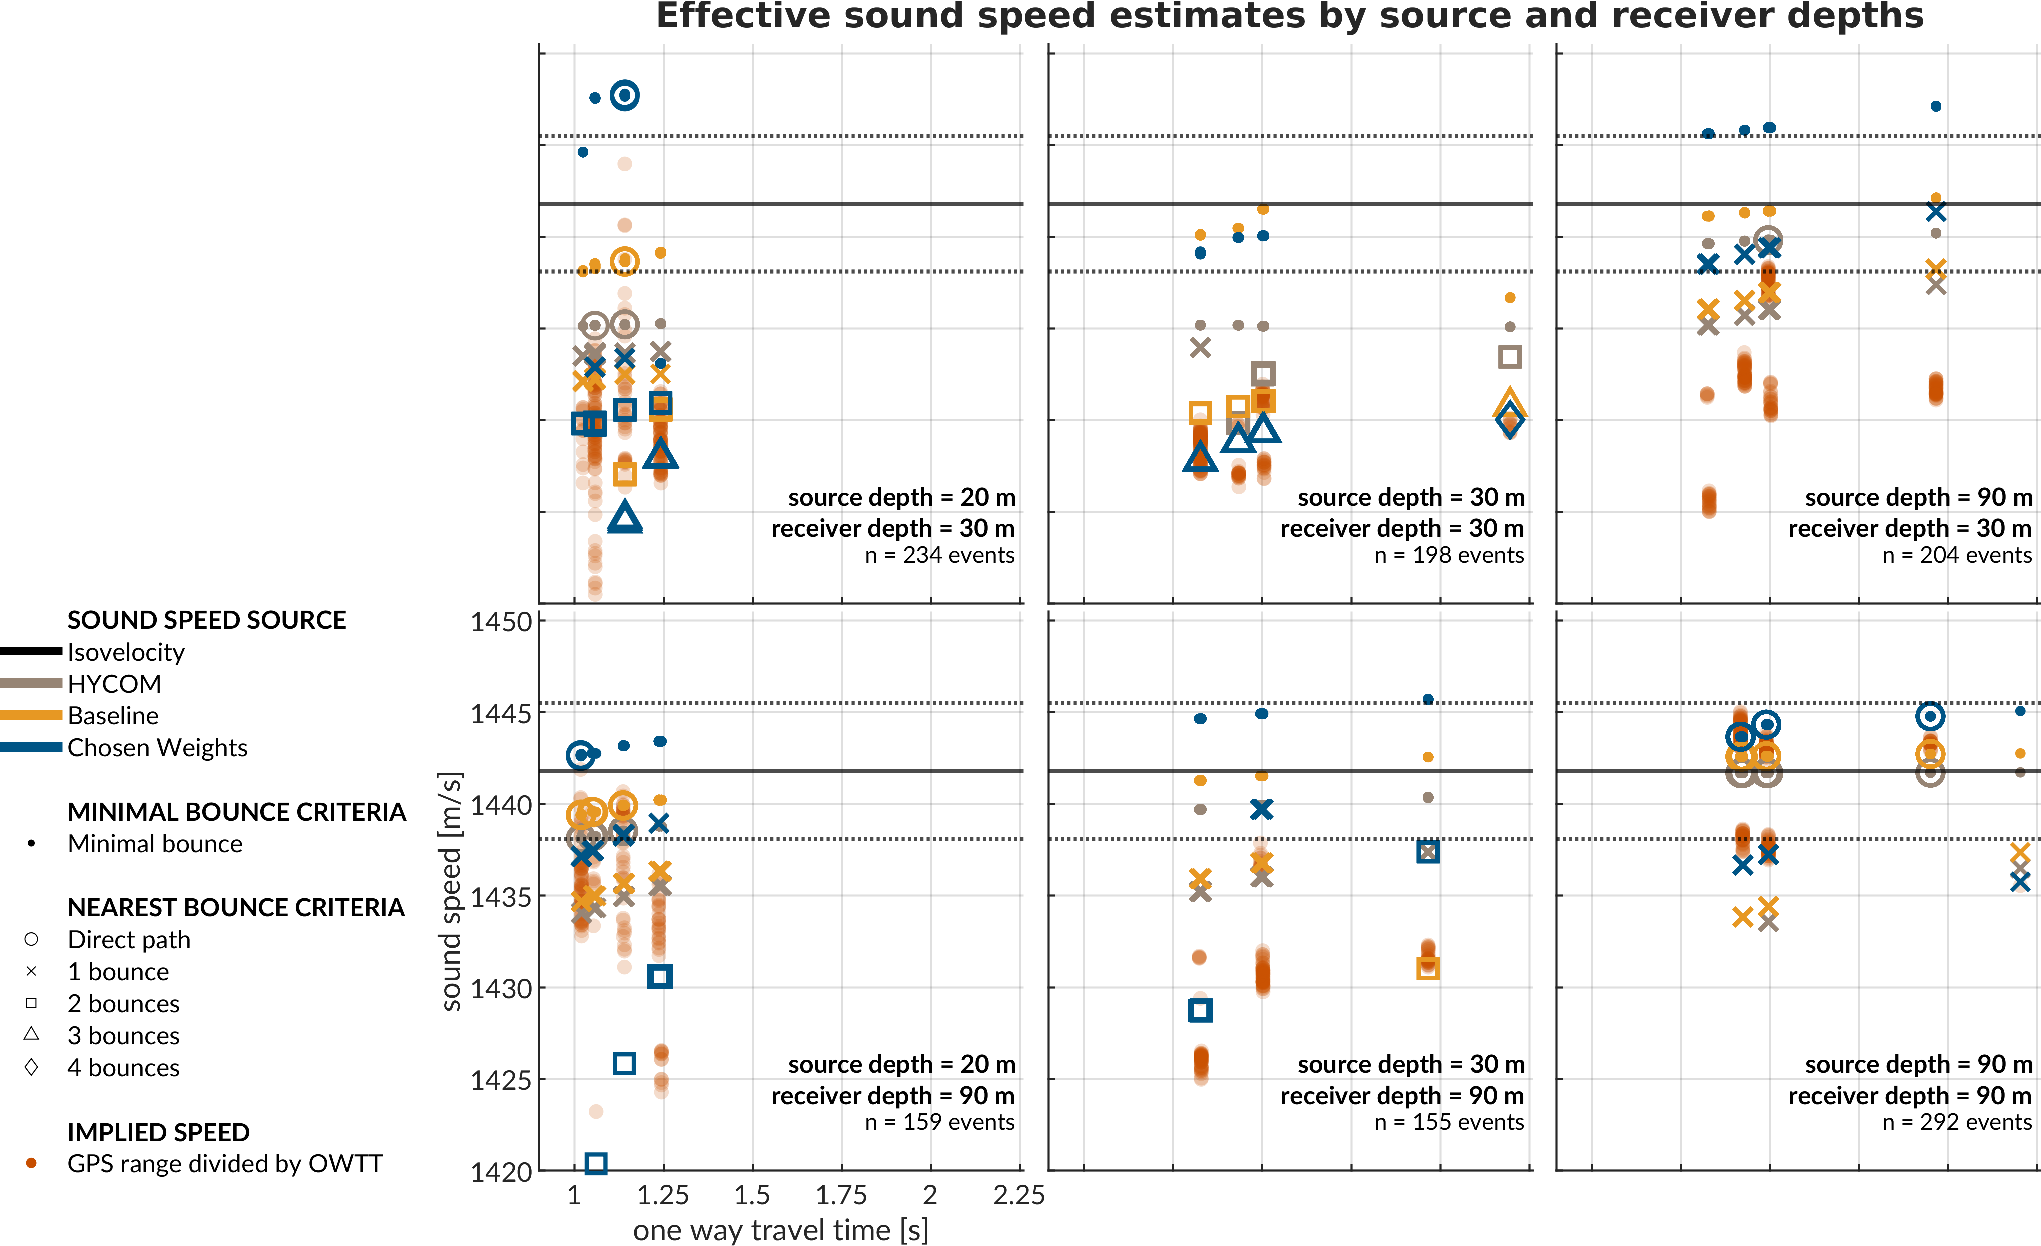
\includegraphics[width=\columnwidth]{figs/gvel-txrxdepth-wIso-wGPS.pdf}
\caption{A post-processing comparison of effective sound speed predictions for all beacon-to-beacon events. The rows share receiver depth; the columns share source depth. The recorded travel time is on the x-axis and the predicted effective sound speed is on the y-axis. The sound speed source is indicated by color. The isovelocity is shown as the mean $\pm$ the standard deviation. The minimal and nearest bounce criterion are distinguished by different marker shapes, compared to the separately colored red dots showing the implied calculation.}
\label{fig:gvel-post}
\end{figure}

The goal of the effective sound speed prediction is to converge towards the implied sound speed, i.e. the GNSS-derived range divided by the recorded travel time.
As the environmental and ray filtering method become better representations of the real ocean, the lower the expected mismatch is between the implied and estimated effective sound speeds.

The various sound speed inputs\textemdash isovelocity aside\textemdash not only modify the predicted effective sound speed, as seen by the colored vertical offsets, but often classify a distinct number of bounces.
HYCOM sees the most direct and one bounce multipath structures, lending a bias for faster speeds; the weighted SSP sees the most double and triple bounces, favoring slower speeds; the baseline sound speed exists in between.
Very rarely is the multipath structure classified as a direct path, where the MBC and NBC would prediction overlap.
In fact, the higher the multipath classification, the more accurate the sound speed prediction is, likely driven by a tighter or even sparser bundle of rays.
\llabel{1.19} Discontinuities in multipath classification provide initial evidence for its importance to a smoothly varying group velocity, as shown in the cluster of 30 to 30 m transmissions in \ref{fig:gvel-post}, where HYCOM jumps from one to two classified bounces amidst the baseline SSP and weighted SSP smoothly increasing while consistently seeing two and three classified bounces, respectively.
Of course, the prediction deteriorates with cross-layer transmissions across the duct, but not to the same degree at which eigenrays could not be found for the weighted SSP in section \ref{sec:eigenrays}.
The evidence suggests that the grid based method provides a useful amount of redundancy to resolve similar enough eigenrays.

It is useful to think about in what case the isovelocity\textemdash or any isovelocity framing\textemdash would have been appropriate.
The transmissions from shallow to shallow receiver would may have matched the default configuration of 1430 m/s.
The isovelocity contrived for this paper, 1441.8 m/s, best matches the transmissions from 90 to 90 m.
The one from \citet{Graupe2019}, 1450 m/s, would have had a systemic overestimation.
In addition, over the course of the four day experiment, the local maxima of the Beaufort Lens changed from roughly 1447 m/s at 40 m to 1442 m/s at 60 m.
Given that implied sound speeds just for beacon-to-beacon events span 1420 to 1445 m/s, it is safe to say that a nominal sound speed would sacrifice pseudorange accuracy somewhere, and that an adaptive approach is necessary even for short and/or small scale operations in the Beaufort Lens.

\subsection{Pseudorange error metrics}

Pseudorange estimation plays an important role in trilateration.
Fig. \ref{fig:rangeError} shows the directional pseudorange error ``footprints'' for the four sound speed inputs with the NBC approach, separated by source and receiver depth configurations.

\begin{figure}[!ht]
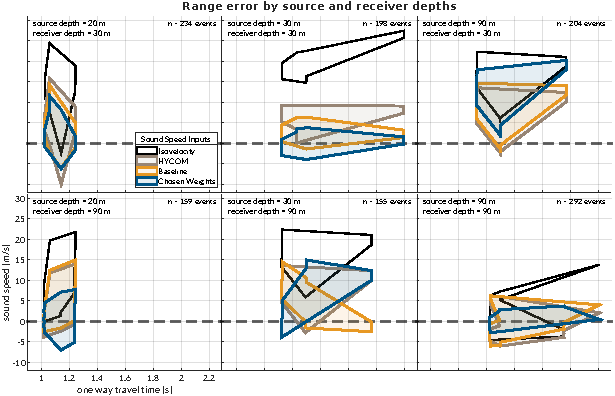
\includegraphics[width=\columnwidth]{figs/range-error-allMethods.pdf}
\caption{The post-processed pseudorange error; the rows share receiver depth; the columns share source depth. The dashed gray line shows no error. The shaded region connects the range performance across all events.}
\label{fig:rangeError}
\end{figure}

The weighted SSP range error generally has the smallest and most zero-centered footprint.
The one case it does not is for the source-receiver pairings between 30 and 90 m in depth.
The increased error for these is most likely driven by the computational artifacts encountered when propagating through the steep sound speed gradients of the lens and through the shadow zone.
All other source depth pairings are significantly improved using the chosen weights compared to HYCOM or the baseline.

When using a linear scaling to convert travel time into range, any offset between the assumed sound speed and the horizontal group velocity produces unconstrained error with increasing receiver distance, whereas an adaptive estimate would exhibit no such trend.
This is easily observed in the same-layer links, i.e., 30 to 30 m and 90 to 90 m.
In cross-layer links, the isovelocity does not perform better but tends to exaggerate or flip the footprint created adaptively.

The improvement from MBC to NBC is most evident for the data-driven sound speed; while the HYCOM SSP improves from a median absolute range error of 6.41 to 4.61 m, the baseline SSP improves from 10.30 to 2.27 m, and the weighted SSP improves from 13.28 to 2.12 m.
In comparison, the isovelocity has a median error of 13.09 m.
The order of magnitude improvement in the ducted SSPs demonstrate the effectiveness of the NBC algorithm exploiting the observed multipath conditions.

\llabel{1.23} There is one example that helpfully illustrates the improvement brought upon by bounce classification.
For transmissions between North and South at 30 m, the OWTT spread is 2.1958 to 2.1963 s; the GNSS-tracked distance is 3138.54 to 3140.87 m; and the implied effective sound speed is 1429.3 to 1430.1 m/s.
For these transmissions, the weighted SSP and the MBC approach produce a pseudorange error of -1491 m, as the effective sound speed is dominated by bottom bounce arrivals with much greater travel times.
The NBC approach categorizes this same record as a quadruple surface bounce, reducing the pseudorange error to less than a meter.
Comparatively, the NBC approach for HYCOM and the baseline SSP produce pseudorange errors of 8.30 and 2.39 m, respectively. 
There is strong evidence to suggest that the sound speed and multipath fidelity codependently improve localization accuracy.

\clearpage
\section{Trilateration for ICEX20 field data}\label{sec:trilat}

To overcome potentially intermittent acoustic communication, the operational paradigm of the ICNN computes corrections relative to the trilaterated position estimates transmitted by the vehicle, rather than transmitting the updated positions themselves.
The reliability of the correction is directly linked to how accurately the travel time measurements are converted to pseudoranges.
This section aims to resolve that tension by reevaluating the trilateration results with respect to the MBC and NBC algorithms.
The MBC/NBC effective speed predictions were tracked independently for each source-receiver pair; although the sound speed was expected to be locally smooth near a given receiver, no such assumption was enforced between distinct acoustic links.

\subsection{Re-positioning beacon to beacon events}

When the beacons ran as virtual vehicles, the ICNN did not have access to that buoy's GPS data stream except for what was sent via digital acoustic message.
The static nature of the experiment means that the initial estimate transmitted to the ICNN was in fact a ground truth position.
Therefore, a distribution of corrections from the ICNN, as shown in Fig. \ref{fig:trilat-beacon}, reflects positioning accuracy.
The NBC clearly outperforms the MBC, with almost 80\% of the corrections below 6 meters and the median within the deployed GNSS puck precision of 3 meters.
By contrast, the MBC shows roughly 20\% within the GNSS puck precision, and separate peaks from 9--12 meters and 21--27 meters.
This trimodal nature reflects the distribution of reflections on the ice surface.

\begin{figure}[!ht]
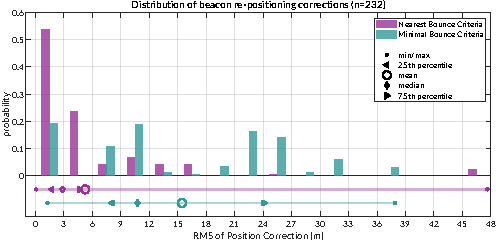
\includegraphics[width=\textwidth]{figs/beacon-trilat-stat.pdf}
\caption{Trilateration events; however, 264 entries are 2-beacon solutions, 22 are 3-beacon, and 2 are 4-beacon. When limited to only two ranging circles, the trilateration chooses the closer of the two intersection points. The x-axis is cut off at the upper limit for the NBC algorithm.}
\label{fig:trilat-beacon}
\end{figure}

In several events, the MBC is unable to accurately estimate the effective sound speed for one of the acoustic links, leading to a large positioning error.
The NBC, however, better resolves an approximation of the acoustic path.
For example, in some trilateration solutions for the Eastern buoy, the MBC shows a correction of more than a kilometer; the NBC is two orders of magnitudes less.

\subsection{Re-navigating AUV \emph{Macrura}}

Up to this point, pseudorange estimation and localization have been evaluated on GPS-linked beacon-to-beacon connections to validate the NBC algorithm.
This analysis ports the MBC and NBC algorithms to re-navigate the AUV \emph{Macrura}.

In comparison to the modem experiment, the AUV data clearly exhibit instances where a receiver detects the same transmission more than once.
This is not surprising considering the complex multipath provided by the Beaufort Lens.
The 11 hour vehicle mission contains 3,260 transmissions, 12,938 total detections, and 4,704 successful receptions.
Allowing receptions with PSK errors would almost double the number of recorded multipath arrivals exploited for positioning, if a real-time solution could correctly parse paths from different arrivals in the same thirty-second cycle.
Thus it remains a future endeavor to explore how failure mode information from acoustic modems could be used to identify unsuccessful but otherwise trustworthy arrivals to augment trilateration samples.

The following performance analysis is constrained to what the vehicle acted on in real-time.
AUV \emph{Macrura} and the ICNN ran an adaptive depth behavior to maintain acoustic communication on the insight that cross-layer links were more likely to fail than same-layer ones.
Accordingly, the vehicle dove deeper than 50 meters about 20\% of the time it was underway.

In contrast to the modem tests, where position correction illustrated re-positioning accuracy, the re-navigation corrections are less valuable in the absence of GNSS ground truth.
The correction magnitude necessarily depends on the vehicle's internal navigation estimate, which is prone to larger errors from sensor drifts, ocean currents, and other error not captured in the hydrodynamic model.
Thus, larger corrections are not necessarily indicative of worse performance.
Navigation accuracy is better described by trilateration error, the RMS of the remaining pseudorange errors from each acoustic link.

Fig. \ref{fig:trilat-auv} shows the correction magnitudes and trilateration errors for events with three or more receptions during AUV operations.
Whereas the MBC has a fairly bimodal nature, with peaks centered around 10--15 and 35--40 m, the NBC favors smaller corrections, from 5--20 m, and has a long tail.
The distribution of corrections are much larger than the distribution of RMS error.
It is apparent that, while both methods are quite successful, there is strong evidence that the NBC achieves single meter accuracy.

\begin{figure}[!ht]
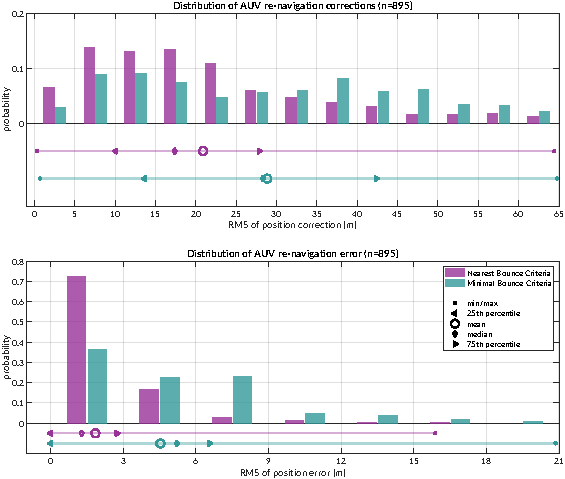
\includegraphics[width=\textwidth]{figs/auv-trilat-stat.pdf}
\caption{Distribution of vehicle re-navigation corrections (top) and error (bottom) computed in post-processing for the Minimum and Nearest Bounce Criterion.}
\label{fig:trilat-auv}
\end{figure}

\subsection{Investigating potential GNSS noise}
\llabel{1.7}

The fact that the bulk of the best performing re-navigation error exists within the precision of the GNSS unit deployed invites a further look into GNSS noise.
In the Arctic, GNSS performance worsens due to poor constellation coverage, larger ionospheric effects, and multipath interference.
The National Security Implications of Climate Change for U.S. Naval Forces \citep{NAP12914} details some of the limitations of the Global Positioning System (GPS) at polar latitudes.
Radio infrastructure that provides position corrections and references does not regularly extend to polar regions.
The effect is minor for surface platform navigation \textemdash roughly 15 m of horizontal precision has been displayed at the North Pole\textemdash but is significant enough to register against the modem's detected travel times.
Fig. \ref{fig:gps-drift-example} zooms in on the GNSS and OWTT noise relative to the ice movement for two pairs of modem buoy connections.
The two panels indicate the GPS drift as $\delta R = \sqrt{\delta x^2 + \delta y^2}$ and temporal drift, $\delta t$, relative to the median OWTT recorded between the two modems.
The dashed line is scaled by a group velocity of 1440 m/s, such that if there were ideal sensor measurements with no drift, all events should exist on or near the line.

\begin{figure}[h!]
	\centering
	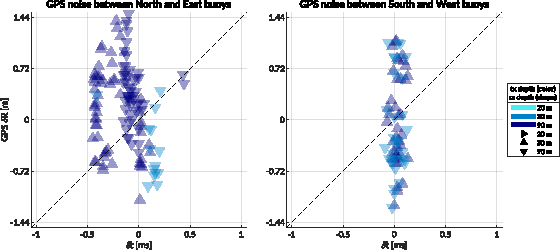
\includegraphics[width=\columnwidth]{figs/gps-drift-example.pdf} 
	\caption{A comparison of GPS drift (y-axis) versus OWTT drift (x-axis) for corners of the ICNN network with different source depths.}
	\label{fig:gps-drift-example}
\end{figure}

The top panel shows the connections between the North and East buoys.
The clusters scaling along the 1440 m/s guideline suggest relative ice movement picked up by both GNSS and OWTT.
But the vertical distribution across many arrival time bands is indicative of the GNSS fluctuations in precision, or noise.
Some minor offsets between these vertical bands relate to different operational configurations of source and receiver depth.
The idea of GNSS noise relative to OWTT is further indicated by events between two other buoys, South and West.
The relatively thin time window suggests these buoys are moving in a more rigid ice floe and that there is minimal impact by source and receiver depth on the spread of OWTT.
Yet, the vertical distribution, spanning almost 4 meters, cannot be explained by time differentials due to acoustic scattering, multipath, and/or environmental microstructure.
This conclusion corroborates the vertical spread of implied effective speeds in Fig. \ref{fig:gvel-post}.

\clearpage
\section{Discussion}

Underwater navigation research is broadly motivated by acquiring GNSS-like navigation in GNSS-denied conditions.
Accurate range estimation is essential to mitigating error.
Current approaches for underwater acoustic navigation simplify the non-linear relationship between a SSP and timefronts with a determinstic sound speed.
Thus, the conversion of travel time into distance can be pre-conditioned for error and error growth over the course of a vehicle mission.
This work introduces a lightweight stochastic prediction of an effective sound speed along the path between source and receiver, retooling arrival methods generally deemed too complex or labor intensive for real-time.
We assume that the effective sound speed would be a locally smoothly varying function with respect to operational conditions\textemdash horizontal and vertical differences and rate of difference between source and receiver.
The field-tested approach, the minimal bounce criteria, facilitated a successful AUV recovery in a total ice-covered, double ducted environment.
The accuracy of the MBC was validated against GPS-linked beacon-to-beacon communications.
Given a consistent bias towards overestimation, an improved algorithm, the nearest bounce criteria, was developed on the insight that multipath structure may play an outsized role in maintaining a smoothly varying effective sound speed.
The NBC was developed with field data and reevaluated on vehicle data, achieving a position accuracy and precision that rivals that of the deployed GNSS puck.

A key insight for both approaches was seeking an eigenray ensemble around an estimated location instead of seeking to unambigously match arrivals.
The ensemble diversified the simulated multipath possibilities to better capture the actual multipath recorded.
In this way, the solution exploits multipath, generally viewed as a source of uncertainty, as a new dimension of information to improve localization accuracy.
Based on the navigation and re-navigation results of our AUV deployment in the ice-covered Beaufort Sea, we conclude that embedding a model-aided prediction of the effective sound speed has an outsized benefit to minimizing trilateration error, and that our approach sufficiently resolves the acoustic timefronts for an unpredictable, complex propagation environment like the double ducted Beaufort Lens.

There are many avenues through which this approach can be further refined and tested for field operations.
Amongst them is defining the uncertainty grid for BELLHOP via stochastic or data-driven measures such as the distance traveled by the AUV between ICNN updates or the magnitude of the position corrections by the ICNN.
Another is to entirely remove the seeded range and instead rely on the submerged asset's depth and recorded OWTT to find high probability fields in range.

The relatively simple nature of this approach suggests it is transferable to other environments, spatio-temporal scales, and platforms.
While it is likely a particular quirk of the Beaufort Lens that filtering for reflection alone can produce a horizontal effective speed that compensates for ray refraction and reflection, it is trivial to filter along other ways, like number of turning points, to create a more diverse and informed set of multipath timefronts.
Though the majority of re-navigation results are within single-meter accuracy, future work can examine how constellations of more LBL beacons can extend the operational domain without adding an undesirable amount of error.
One possibility is that, during a mission, ICNN-like LBL implementions use a comparison of the GNSS self-position and acoustic positioning to invert for the ocean volume, linking how vertical and horizontal sound speed structure impact transmission integrity.
\llabel{1.20} A fast tomographic estimate \citep{deffenbaugh_optimal_1997,Elisseeff2002}, along with its uncertainty, can be continuously communicated to assets underway to maintain contact or enable adaptive sampling.
In this sense navigation and tomography converge on the same set of component technologies\textemdash position estimation, sound speed parameterization estimation, ray path identification, and vehicle path optimization.

Spatio-temporal variability is a serious challenge for accurate real-time ranging.
On one hand, the effectiveness of eigenray filtering algorithm is likely only challenged by the valid operational scales of a range independent propagation environment.
Longer range experiments may provide more time for eigenray filtering.
A bootstrapping approach that filters eigenrays for several randomly generated internal wave spectrums may compensate for otherwise unknowable spatio-temporal variability.
The model-aided component to the eigenray filtering is compatible with vertical slices from any physically driven ocean model.
But in the long run, more accurate and higher resolution global circulation models are needed to properly resolve features that alter ducted propagation at the scales discernible to an acoustic modem.
Through-the-sensor methods can resolve local features but would require a degree of information sharing not readily supported on the acoustic channel for large scale variability.
But addressing the spatial and temporal scales of what can be solved deterministically and what must be solved stochastically imposes a resolution constraint that is at odds with computational overhead for real-time operations.
Resolving features inaccurately, or with a false sense of confidence, could be more harmful than contextualizing the limitations of a range independent propagation over realistic bathymetry.
Given that AUV operations are often on smaller spatial and temporal scales, the added benefit of a gridded model is quite small, and for features like the Beaufort Lens, not well resolved.

\llabel{1.1}
The methods presented in this paper, including the software projects \citep{,Benjamin2010,schneider2015dynamic,schneider_unified_2010}, are open source and platform agnostic.
Large AUVs, often large enough to support long duration and/or deep sea missions, would benefit from including diurnal or tidal effects for ranging.
Gliders, though generally low power and memory, have been equipped with acoustic modems.
Their inability to maintain position within a region of reliable acoustic path makes the impact of an environmentally adaptive pseudorange estimation disproportionately positive.
The exact adjustments to the ensemble eigenray filtering are predicated on the expected sound speed conditions and acoustic arrival structure; the problem is ripe application for other simulation testbeds or machine learning methods.
The continued development of embedded acoustic processing on heterogenous platforms is fundamental to support a universal underwater navigation scheme comparable to GNSS.

% ================================================== %
% \begin{figure}[ht]
% \includegraphics[width=\reprintcolumnwidth]{figsamp.jpg}
% \caption{\label{fig:FIG1}{Caption here.}}

% \raggedright
% {\color{red}
% Note: The only figure formats allowed are the following:
% .pdf, .ps, .eps, or .jpg. Figure files must be named in this fashion:
% Figure\#.xxx, where ``\#'' is the figure number and ``xxx'' is the file format
% (Figure1.eps, Figure2.jpg, Figure3a.ps, Figure3b.ps, etc).
% }

% [For these sample pages we have used only figsamp.jpg for convenience]
% \end{figure}
% ================================================== %
\FloatBarrier
\clearpage
\begin{acknowledgments}
We acknowledge the significant operational effort spearheaded by the LAMSS ICEX20 team and all our collaborators.
Bhatt was funded by a National Defense, Science, and Engineering Graduate Fellowship.
This work was supported by the Office of Naval Research 322-OA under ICEX20 (N00014-17-1-2474) and Task Force Ocean (N00014-19-1-2716).
\end{acknowledgments}

\bibliography{sampbib}